\documentclass[twocolumn]{article}

\usepackage[english]{babel} 


\usepackage[utf8]{inputenc}
\usepackage[T1]{fontenc}
\usepackage{lmodern}
\usepackage{amsmath}
\usepackage{verbatim}
\usepackage{amssymb}
\usepackage{mathtools}
\usepackage{enumitem}
\usepackage{float}
\usepackage{titlesec} 

\titleformat{\subsection}[runin]{\normalfont\large\bfseries}{\thesubsection}{1em}{}

\setlength{\parindent}{0pt}

\begin{document}

\begin{center}

\Large{\textbf{MLDS: Homework 5}} \\
\textsc{\large{Andraž De Luisa}} \\
\vspace{6pt}
\small{\today}

\end{center}

Implement support vector regression with two kernels: polynomial $\kappa (x, x') = (1 + x x')^M $ and RBF kernel: $\kappa (x, x') = \exp(- \frac{||x - x'||^2}{2 \sigma^2})$.

\subsection*{Task 1}

Figure \ref{fig:sine} shows the fitting of the support vector regression model on the sine dataset, with two different kernels: a polynomial and a RBF kernel. The values of the kernel parameters are not optimal with respect to any measure, I have just chosen such values that visually fit well to the actual sine values from the data. A smaller value of the degree M in the polynomial kernel would result in a flattened curve, while a higher M would cause a clear overfit. A similar behaviour could be seen with the RBF kernel, with the lost of smoothness (i.\ e. overfit) for lower $\sigma$, and a flattening for higher ones. The margin $\epsilon = 0.5$ was chosen in such way to obtain a sparse model (less than 10\% of support vectors in this case).

\begin{figure}[ht]
    \centering
    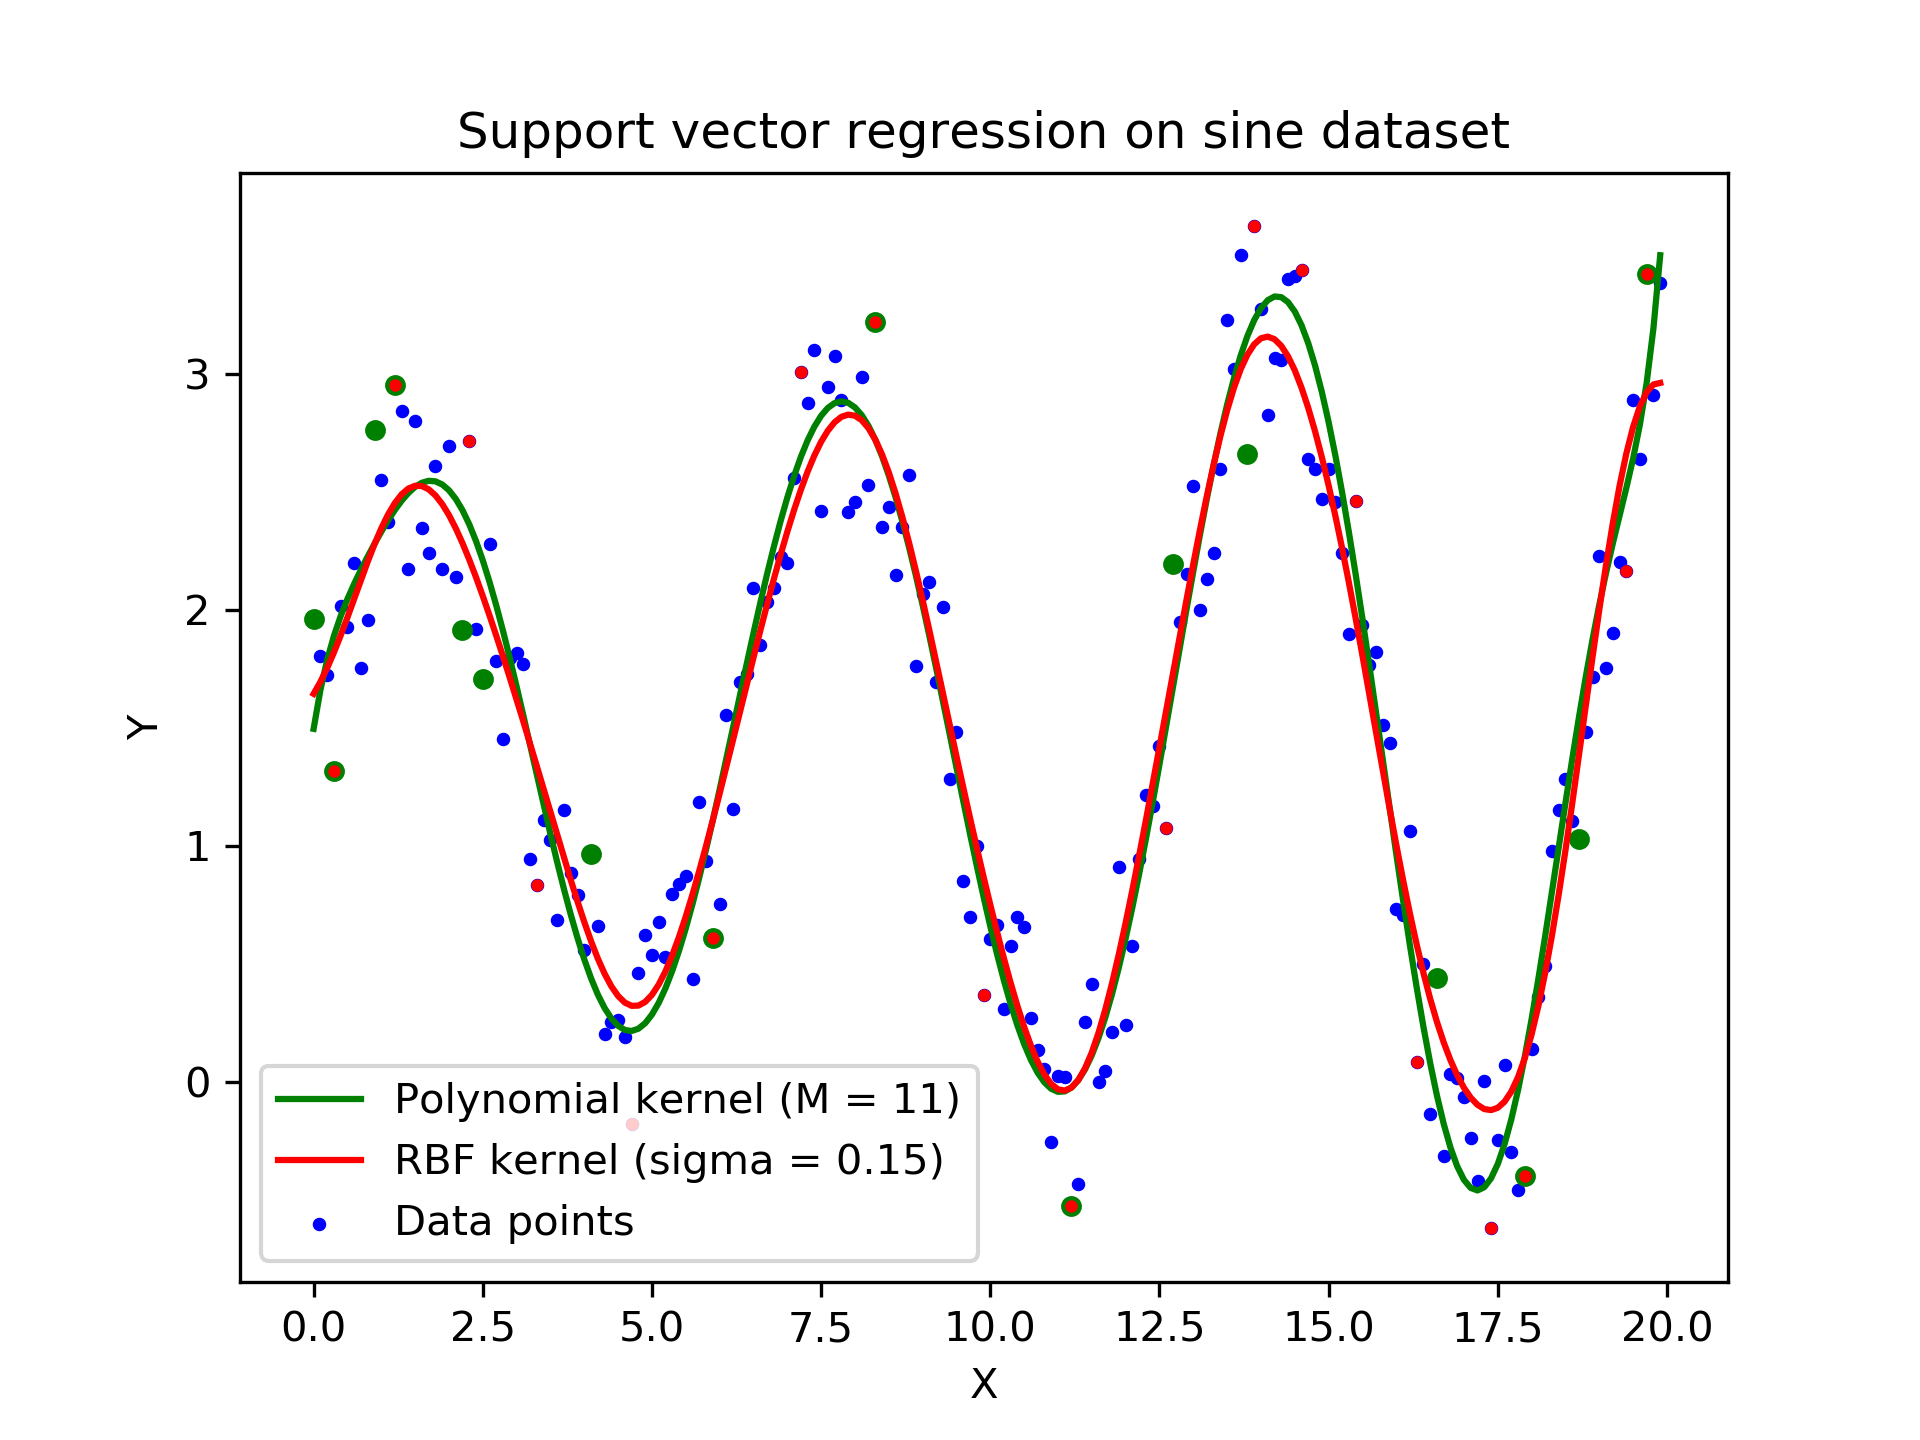
\includegraphics[width=.4\textwidth]{sine.png}
    \caption{Support vector regression with a polynomial and a RBF kernel, both with regularization parameter $\lambda = 0.01$. Support vectors for each model are marked.}
    \label{fig:sine}
\end{figure}

\subsection*{Task 2}

Figures \ref{fig:house_pol} and \ref{fig:house_rbf} show the evaluation of the support vector regression with polynomial and RBF kernel on the test data from the housing dataset. As the measure of predictive performance the RMSE (rooted mean squared errors) was used, both in parameter optimization and model evaluation. Both figures present a comparison between a fixed regularization parameter $\lambda  = 1$ and the best $\lambda$ for each kernel parameter (M or $\sigma$), set with internal 5-fold cross-validation. In figure \ref{fig:house_pol} just the degrees up to 4 are shown, because the errors grow too much from degree 5 onwards due to overfit. With both kernels the CV estimation of the regularization parameter seem to slightly improve the performance of the model, but we can't really make any conclusion about it because of the uncertainty involved.

\begin{figure}[ht]
    \centering
    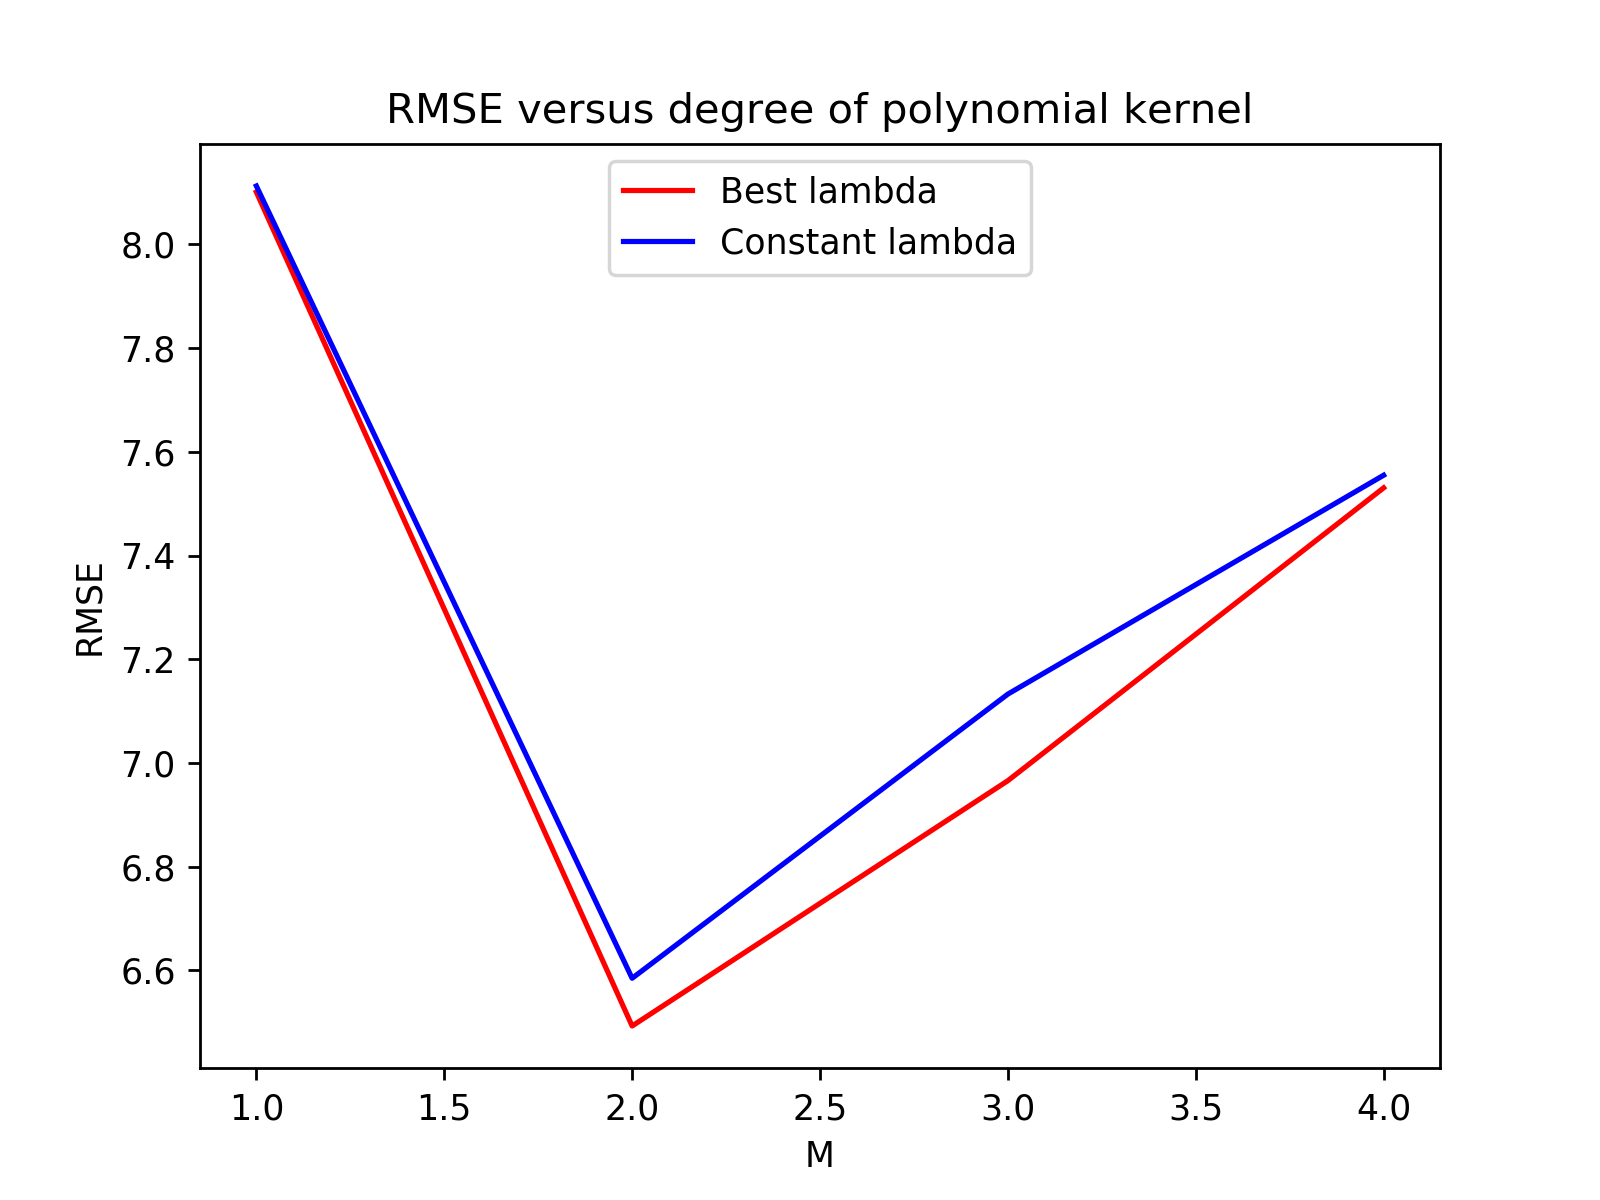
\includegraphics[width=.4\textwidth]{housing_pol.png}
    \caption{Polynomial kernel}
    \label{fig:house_pol}
\end{figure}

\begin{figure}[ht]
    \centering
    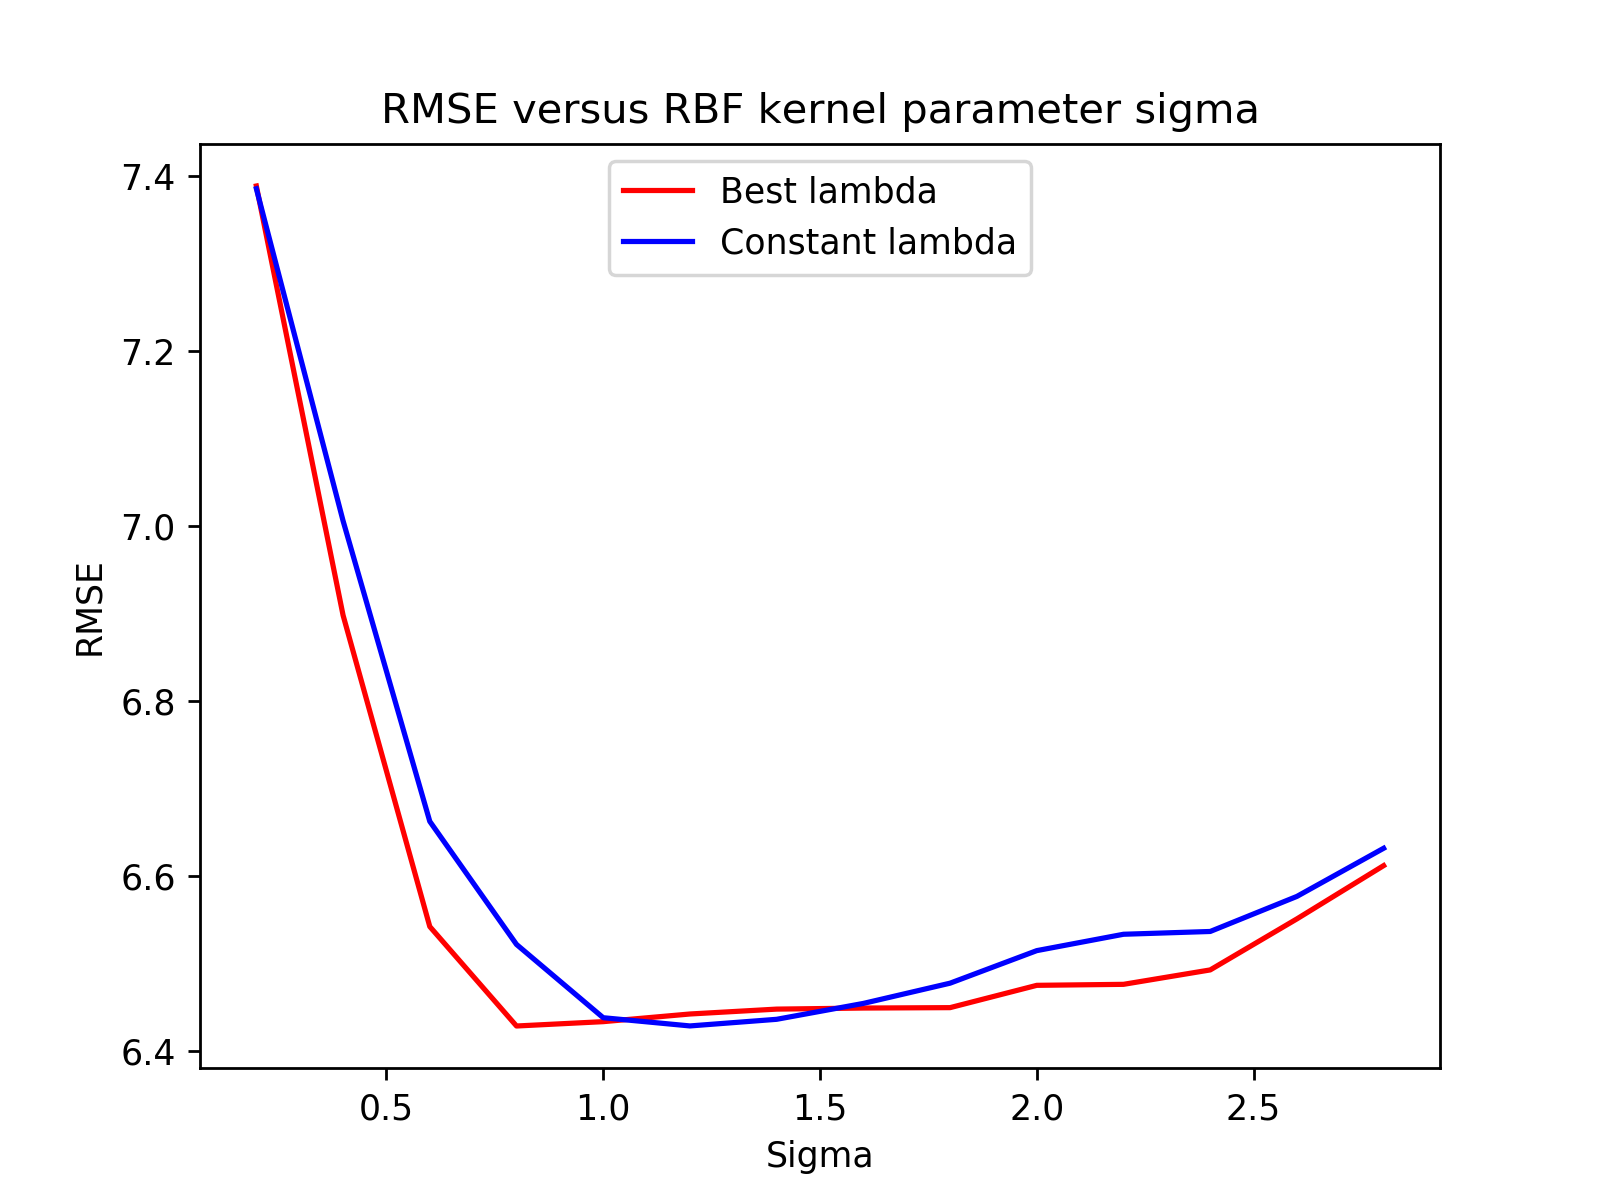
\includegraphics[width=.4\textwidth]{housing_rbf.png}
    \caption{RBF kernel}
    \label{fig:house_rbf}
\end{figure}

\end{document}